% Options for packages loaded elsewhere
\PassOptionsToPackage{unicode}{hyperref}
\PassOptionsToPackage{hyphens}{url}
%
\documentclass[
  11pt,
]{article}
\usepackage{lmodern}
\usepackage{amssymb,amsmath}
\usepackage{ifxetex,ifluatex}
\ifnum 0\ifxetex 1\fi\ifluatex 1\fi=0 % if pdftex
  \usepackage[T1]{fontenc}
  \usepackage[utf8]{inputenc}
  \usepackage{textcomp} % provide euro and other symbols
\else % if luatex or xetex
  \usepackage{unicode-math}
  \defaultfontfeatures{Scale=MatchLowercase}
  \defaultfontfeatures[\rmfamily]{Ligatures=TeX,Scale=1}
\fi
% Use upquote if available, for straight quotes in verbatim environments
\IfFileExists{upquote.sty}{\usepackage{upquote}}{}
\IfFileExists{microtype.sty}{% use microtype if available
  \usepackage[]{microtype}
  \UseMicrotypeSet[protrusion]{basicmath} % disable protrusion for tt fonts
}{}
\makeatletter
\@ifundefined{KOMAClassName}{% if non-KOMA class
  \IfFileExists{parskip.sty}{%
    \usepackage{parskip}
  }{% else
    \setlength{\parindent}{0pt}
    \setlength{\parskip}{6pt plus 2pt minus 1pt}}
}{% if KOMA class
  \KOMAoptions{parskip=half}}
\makeatother
\usepackage{xcolor}
\IfFileExists{xurl.sty}{\usepackage{xurl}}{} % add URL line breaks if available
\IfFileExists{bookmark.sty}{\usepackage{bookmark}}{\usepackage{hyperref}}
\hypersetup{
  pdftitle={Variation in histone configurations correlates with gene expression across nine inbred strains of mice},
  hidelinks,
  pdfcreator={LaTeX via pandoc}}
\urlstyle{same} % disable monospaced font for URLs
\usepackage[margin=1in]{geometry}
\usepackage{graphicx}
\makeatletter
\def\maxwidth{\ifdim\Gin@nat@width>\linewidth\linewidth\else\Gin@nat@width\fi}
\def\maxheight{\ifdim\Gin@nat@height>\textheight\textheight\else\Gin@nat@height\fi}
\makeatother
% Scale images if necessary, so that they will not overflow the page
% margins by default, and it is still possible to overwrite the defaults
% using explicit options in \includegraphics[width, height, ...]{}
\setkeys{Gin}{width=\maxwidth,height=\maxheight,keepaspectratio}
% Set default figure placement to htbp
\makeatletter
\def\fps@figure{htbp}
\makeatother
\setlength{\emergencystretch}{3em} % prevent overfull lines
\providecommand{\tightlist}{%
  \setlength{\itemsep}{0pt}\setlength{\parskip}{0pt}}
\setcounter{secnumdepth}{-\maxdimen} % remove section numbering

\newcommand{\beginsupplement}{%
        \setcounter{table}{0}
        \renewcommand{\thetable}{S\arabic{table}}%
        \setcounter{figure}{0}
        \renewcommand{\thefigure}{S\arabic{figure}}%
     }

\usepackage{natbib}

\usepackage{setspace} \doublespacing

\usepackage{fancyhdr}
\pagestyle{fancy}
\lhead{Tyler, Spruce, et al.}
\rhead{Epigenetic variation in nine inbred mouse strains}

\bibliographystyle{genome_research}
\ifluatex
  \usepackage{selnolig}  % disable illegal ligatures
\fi

\title{Variation in histone configurations correlates with gene
expression across nine inbred strains of mice}
\author{}
\date{\vspace{-2.5em}}

\begin{document}
\maketitle

Anna L. Tyler\textsuperscript{1,$*$}, Catrina
Spruce\textsuperscript{1,$*$}, Romy Kursawe\textsuperscript{2}, Annat
Haber\textsuperscript{2}, Robyn L. Ball\textsuperscript{1}, Wendy A.
Pitman\textsuperscript{1}, Alexander D. Fine\textsuperscript{1},
Narayanan Raghupathy\textsuperscript{1}, Michael
Walker\textsuperscript{1}, Vivek M. Philip\textsuperscript{1},
Christopher L. Baker\textsuperscript{1}, J. Matthew
Mahoney\textsuperscript{1}, Gary A. Churchill\textsuperscript{1},
Jennifer J. Trowbridge\textsuperscript{1}, Michael L.
Stitzel\textsuperscript{2}, Kenneth Paigen\textsuperscript{1}, Petko M.
Petkov\textsuperscript{1,$\dagger$}, Gregory W.
Carter\textsuperscript{1,$\dagger$}

\textsuperscript{1} The Jackson Laboratory for Mammalian Genetics, 600
Main St.~Bar Harbor, ME, 04609

\textsuperscript{2}The Jackson Laboratory for Genomic Medicine 299
Farmington Ave, Farmington, CT 06032

\(^*\) equal contribution \(^\dagger\) corresponding authors

Running title: Epigenetic variation in nine inbred mouse strains

\pagebreak

\hypertarget{abstract}{%
\section{Abstract}\label{abstract}}

The diversity outbred (DO) mice and their inbred founders are widely
used models of human disease. However, although the genetic diversity of
these mice has been well documented, their epigenetic diversity has not.
Epigenetic modifications, such as histone modifications and DNA
methylation, are important regulators of gene expression, and as such
are a critical mechanistic link between genotype and phenotype.
Therefore, creating a map of epigenetic modifications in the DO mice and
their founders is an important step toward understanding mechanisms of
gene regulation and the link to disease in this widely used resource. To
this end, we performed a strain survey of epigenetic modifications in
hepatocytes of the DO founders. We surveyed four histone modifications
(H3K4me1, H3K4me3, H3K27me3, and H3K27ac), and DNA methylation. We used
ChromHMM to identify 14 chromatin states, each of which represented a
distinct combination of the four histone modifications. We found that
the epigenetic landscape was highly variable across the DO founders and
was associated with variation in gene expression across strains. We
found that epigenetic state imputed into a population of DO mice
recapitulated the association with gene expression seen in the founders
suggesting that both histone modifications and DNA methylation are
highly heritable mechanisms of gene expression regulation. We illustrate
how DO gene expression can be aligned with inbred epigenetic states to
identify putative cis-regulatory regions. Finally, we provide a data
resource that documents strain-specific variation in chromatin state and
DNA methylation in hepatocytes across nine widely used strains of
laboratory mice.

\hypertarget{introduction}{%
\section{Introduction}\label{introduction}}

The development of the diversity outbred (DO) mice
\citep{Svenson:2012hq, churchill2012diversity, 
koyuncu2021cxcl1, kurtz2020diversity, bogue2015collaborative, 
kebede2014insights, keller2019gene} and their sister population, the
collaborative cross (CC) \citep{threadgill2011collaborative, 
threadgill2012ten, durrant2011collaborative, mao2015identification, 
graham2021baseline}, has demonstrated the critical importance of genetic
diversity in our understanding of disease biology. These mice have been
used to investigate the genetic architecture of complex disease
\citep{pmid28592500}, to identify genetic modifiers of Mendelian disease
\citep{takemon2021uncovering}, and to study the effects of genetic
variation on susceptibility to infectious disease
\citep{kurtz2020diversity}. These models have huge potential to uncover
mechanistic insights into multiple aspects of human health and disease.
However, although the genetic diversity of these mice is well
documented, the epigenetic diversity of these mice is relatively
unknown. This gap in knowledge is potentially critical to understanding
mechanisms of gene regulation and its impact on disease in these
important models.

Epigenetic modifications, such as histone modifications
\citep{pmid32671792, pmid29625185} and DNA methylation
\citep{pmid21701563, pmid20720541}, regulate gene expression by
modifying the accessibility of DNA to transcription machinery
\citep{lawrence2016lateral, 
jones2012functions, moore2013dna}. These modifications allow an organism
to develop an array of diverse cell types from a single genome.

Epigenetic modifications also vary across individuals. Studies in humans
\citep{mcvicker2013identification, kang2021genetic}, rats
\citep{rintisch2014natural}, and cattle \citep{prowse2022genetic} have
identified genetic loci associated with variation in histone
modification. Heritable variation in histone modification has also been
linked to variation in gene expression
\citep{kang2021genetic, rintisch2014natural, prowse2022genetic} and
clinical outcomes \citep{kang2021genetic}. Similar studies have
associated heritable variation in DNA methylation to clinical outcomes,
such as immune dysregulation \citep{hawe2022genetic}.

This link between genetic variation and epigenetic variation may be a
critical piece of understanding genetic susceptibility to disease.
Because the majority of disease-associated genetic variants discovered
in humans are in gene regulatory regions, it has been suggested that it
is the regulation of gene expression, rather than alteration of protein
function, that is the primary mechanism through which genetic variants
confer disease risk
\citep{maurano2012systematic, farh2015genetic, pmid21617055, pmid19474294}.
Detailed epigenomic landscapes, therefore, may provide important
mechanistic insight connecting genotype to disease risk.

To address the lack of documented epigenetic variation in the DO/CC
founders, we undertook a strain survey of epigenetic variation in
hepatocytes across the eight founders of the DO/CC mice, as well as
DBA/2J, which, along with C57BL/6J, is one of the founders of the widely
used BxD recombinant inbred panel of mice \citep{Ashbrook:2019bd}.

We assayed four histone modifications: H3K4me3, which is associated with
promoter regions \citep{heintzman2007distinct, pmid15680324}, H3K4me1,
which is associated with enhancer regions \citep{heintzman2007distinct},
H3K27me3, which is associated with polycomb repression
\citep{bonasio2010molecular}, and H3K27ac, which has been associated
with active enhancers and promoters
\citep{creyghton2010histone, heintzman2009histone, rada2011unique}. We
also assayed DNA methylation which is differentially associated with
gene expression depending on its position relative to the gene
\citep{moore2013dna, jones2012functions}. Methylation of DNA in
promoters inactivates the promoters thereby reducing gene expression,
whereas methylation of DNA in insulators inactivates the insulators
thereby increasing expression of the targeted gene
\citep{jones2012functions}.

We used ChromHMM \citep{Ernst:2012ii} to identify 14 chromatin states,
each representing a unique combination of the four histone marks. We
investigated the association between variation in these epigenetic
markers and variation in gene expression across the nine inbred strains.

We extended our analysis into a population of DO mice to investigate the
heritability of histone modifications and DNA methylation with respect
to gene expression. To do this, we imputed the 14 chromatin states and
DNA methylation into the DO mice. We then mapped gene expression to the
imputed epigenetic states to assess the extent to which expression
quantitative trait loci (eQTLs) in the DO were related to variation in
epigenetic modifications.

\hypertarget{results}{%
\section{Results}\label{results}}

Both gene expression and epigenetic state were consistent within each
inbred mouse strain but varied across the strains suggesting strong
genetic regulation of both modalities. This is seen as a clustering of
individuals from the same strain in principal component plots of
transcriptomic and epigenetic features (Fig. \ref{fig:pc_plots}).
Patterns of gene expression (Fig. \ref{fig:pc_plots}A), DNA methylation
(Fig. \ref{fig:pc_plots}B) and individual histone modifications (Fig.
\ref{fig:pc_plots}C-F) clustered in similar patterns, although a
relatively small percent of the variation in the methylome was related
to strain. The three subspecies \textit{musculus} (in red),
\textit{castaneous} (in green) and \textit{domesticus} (all others) were
widely separated suggesting that subspecies structure made up the
majority of the observed variance. The \text{domesticus} strains largely
clustered together. These data provide evidence that epigenetic features
relate to gene expression in a manner that is consistent with the
subspecific origin of the mouse strains \citep{yang2007subspecific}. For
a more detailed visualization of the correlations between strains see
Supplemental Figure \ref{supp_fig:feature_correlation}. Also, note that
all genes used in this analysis were expressed at a minimal level across
the strains (overall mean of 5 TPM), so results do not include data from
non-expressed genes.

\begin{figure}[ht!]
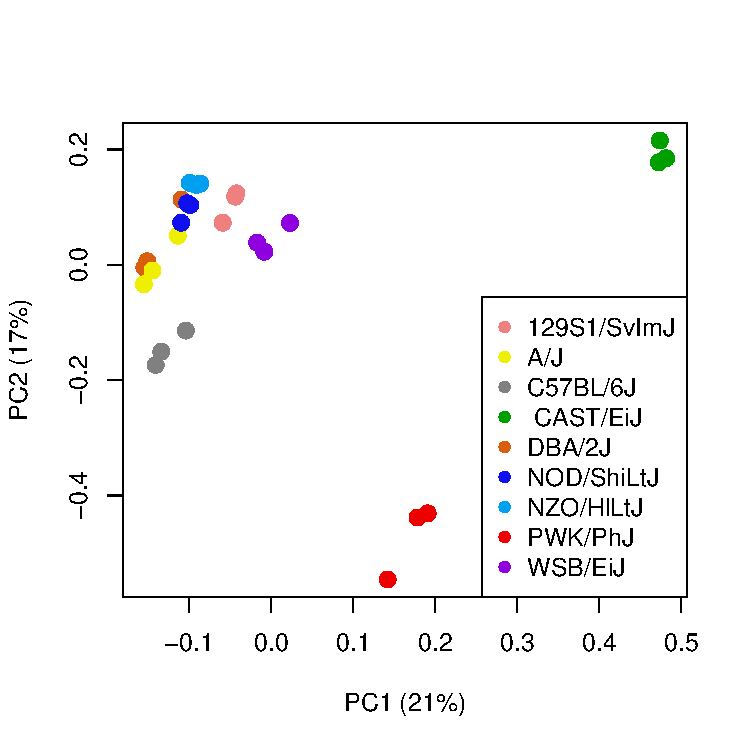
\includegraphics[width=3in]{Figures/Fig1_Decomposition.png} 
\caption{The first two principal components of each genomic 
feature across nine inbred mouse strains. In all panels each 
point represents an individual mouse, and strain is indicated 
by color as shown in the legend at the bottom of the figure. 
Three individuals per strain are shown. Each panel is labeled 
with the data used to generate the PC plot. (A) Hepatocyte 
transcriptome - all transcripts expressed in isolated hepatocytes. 
(B) DNA methylation - the percent methylation at all CpG sites 
shared across all individuals. (C-F) Histone modifications - 
the peak heights of the indicated histone modification for
positions aligned across strains.}
\label{fig:pc_plots}
\end{figure}

\hypertarget{chromatin-state-overview}{%
\subsection{Chromatin state overview}\label{chromatin-state-overview}}

We used ChromHMM to identify 14 chromatin states composed of unique
combinations of the four histone modifications (Fig.
\ref{fig:state_overview}A). We calculated the enrichment of each state
near predicted functional elements in the mouse liver (Fig.
\ref{fig:state_overview}B), and correlated the presence of each state
with gene expression both across genes and across the inbred strains
(Fig. \ref{fig:state_overview}C).

\begin{figure}[ht!]
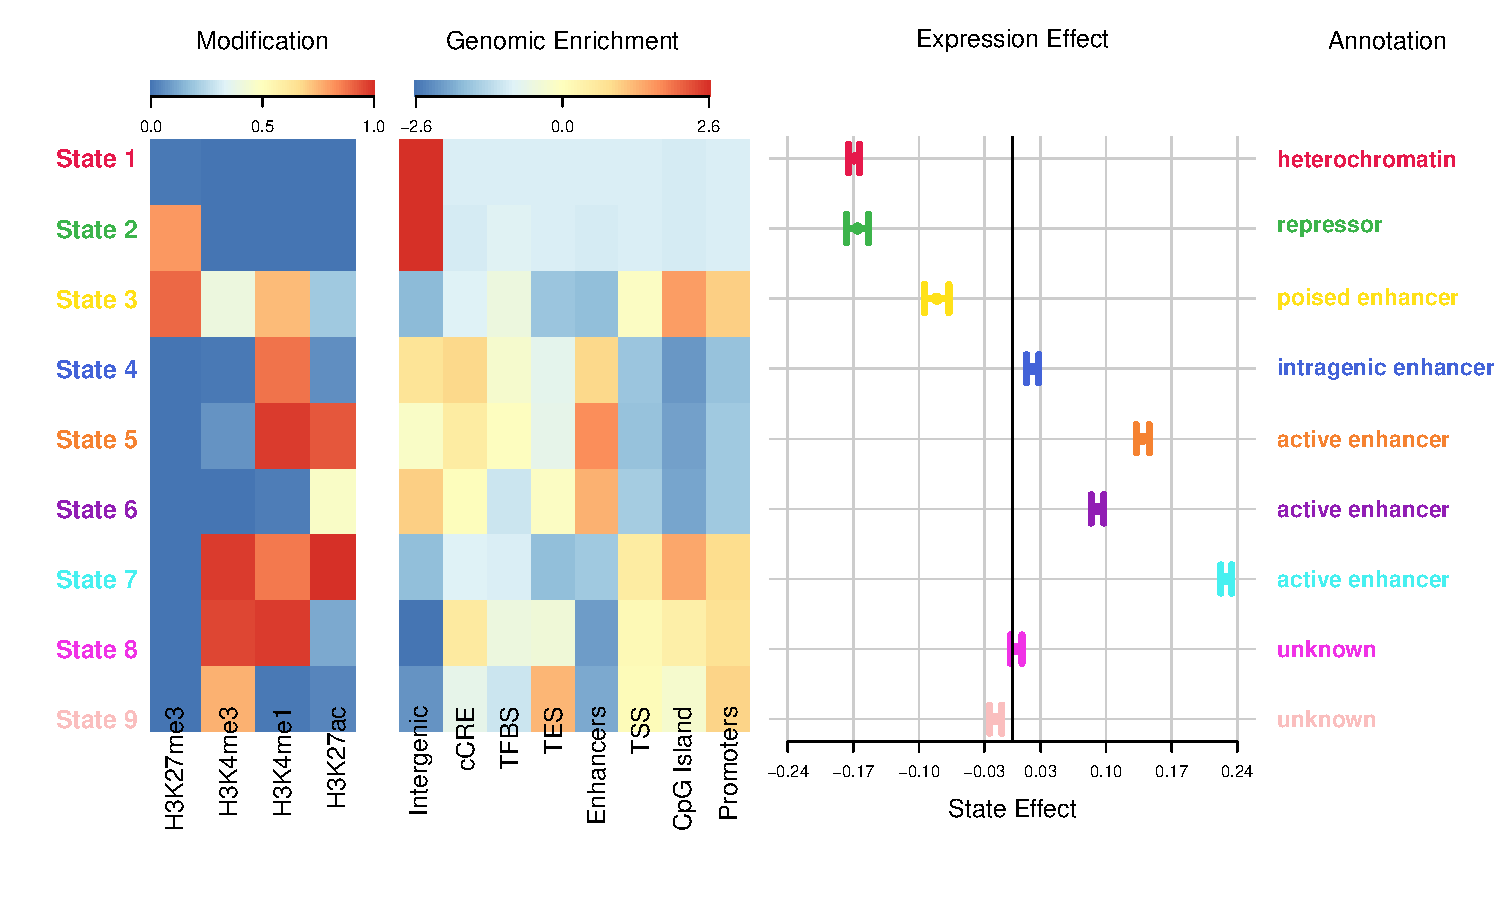
\includegraphics[width=\textwidth]{Figures/Fig2_Overview.png} 
\caption{Overview of chromatin state composition, genomic 
distribution, and association with expression. (A) Emission 
probabilities for each histone modification in each 
chromatin state. Blue indicates the absence of the histone
modification, and red indicates the presence of the 
modification. (B) The distribution of each state around 
functional elements in the genome. Red indicates that the 
state is enriched near the annotated functional element. 
Blue indicates that the state is depleted near the annotated 
functional element. Abbreviations are as follows: 
Enh. = enhancer, Tsd = distal to the transcription start site, 
Tsp = proximal to the transcription start site; Hetero. = 
heterochromatin; FR = flanking region. (C) The association between 
chromatin state variation and gene expression. Bars are colored 
based on the size and direction the state's association with expression. 
Red/blue bars show the associations of chromatin state with gene
expression across strains. Blue-gray bars show the associations of
chromatin state with gene expression across genes. (D) Plausible 
annotations for each state based on genomic enrichments and association
with gene expression. The numbers in parentheses indicate the percent 
of the genome that was assigned to each state. Repress. = repressor.}
\label{fig:state_overview}
\end{figure}

To associate chromatin state with expression across transcripts (Fig.
\ref{fig:state_overview}C blue-gray bars), we calculated the proportion
of each gene body that was occupied by each state in each inbred strain.
We then fit a linear model to associate the proportion of each chromatin
state with the amount of transcription (Methods). We did this separately
in each strain. Some chromatin states, such as State 1 were more
abundant in highly expressed genes, whereas other states, such as State
13, were more abundant in lowly expressed genes.

We compared this correlation to the correlation between chromatin state
and gene expression across strains (Fig. \ref{fig:state_overview}C
red/blue bars) (Methods). To do this, we normalized the expression of
each transcript and the proportion of each chromatin state across
strains (Methods). We then fit a linear model to estimate whether the
proportion of each state varying across strains was associated with gene
expression. For any given transcript, strains with greater proportions
of State 1 had higher expression than strains with lower proportions of
State 1. Through this calculation, we can associate strain variation in
chromatin state with strain variation in gene expression.

In Figure \ref{fig:state_overview}, the states are ordered by their
association with gene expression across strains, which helps illustrate
several patterns. Overall, states that were associated with increased
expression across transcripts were also associated with increased
expression when varying across strains. The state with the largest
negative association with gene expression across strains, State 14, was
the absence of all measured modifications. Other states associated with
reduced gene expression contained the repressive mark H3K27me3. The
states with the largest positive correlations with gene expression all
had some combination of the activating marks H3K4me3, H3K4me1, and
H3K27ac. The repressive mark was less commonly seen in these activating
states.

We used the functional element enrichments to assign putative
annotations to each of the 14 chromatin states (Fig.
\ref{fig:state_overview}D). Except for State 14, all states were
enriched around at least one of the predicted functional elements in
mouse liver (Fig. \ref{fig:state_overview}B). Where there was more than
one obvious enrichment for the state, we used our own associations with
gene expression to narrow down which regulatory label we assigned each
state. Interestingly, the enrichments of these states largely matched
the associations we saw between each state and gene expression (Fig.
\ref{fig:state_overview}C). For example, State 1, which was enriched
around strong enhancers, was the state that was most strongly correlated
with increased expression both across genes, and across strains.
Likewise, States 2-4 were all enriched around active enhancers or
promoters, and were all correlated with increased expression overall.

At the other end of the spectrum, state 13 was enriched around polycomb
repressor marks, as we would expect because it was defined by presence
of H3K27me3, which is associated with polycomb repression. This state
was also correlated with reduced expression both across genes and across
strains.

Many of the states with weaker associations with gene expression, both
positive and negative were most enriched around bivalent promoters. This
suggests that the bivalent promoter class may represent a diverse array
of functional elements with varied effects on gene expression, and that
more detailed experiments investigating the relationship between these
states and gene expression could potentially identify novel chromatin
states influencing expression in these cells.

\hypertarget{dna-methylation-overview}{%
\subsection{DNA methylation overview}\label{dna-methylation-overview}}

To investigate the variation in DNA methylation across the inbred
strains, we examined both strain-specific CpG sites and strain-specific
methylation values. We defined a strain-specific CpG site as one that
was present in all individuals in at least one strain and absent in all
individuals in at least one other strain.

Roughly 17.8\% of all CpG sites were strain-specific ranging from 16\%
to 19\% across the chromosomes. Strain-specific CpG sites were more
commonly present in CAST, PWK, and B6 compared to the other strains
(Fig. \ref{fig:cpg_overview}A), suggesting that these strains have more
DNA methylation overall compared with the other strains.

\begin{figure}[ht!]
\begin{minipage}[c]{0.4\textwidth}
  \includegraphics[width=\textwidth]{Figures/Fig3_CpG_Overview.png} 
\end{minipage}\hfill
\begin{minipage}[c]{0.5\textwidth}
\caption{Overview of strain-specific CpG sites. (A) Boxes 
show proportion of strain-specific CpG sites that are present 
in each strain. Boxes are colored by official strain colors
for ease of visualization. Short names for strains are
indicated below each box. (B) The $log_{10}$(Fold Enrichment)
of CpG sites shared across all strains (green) and those
that are strain-specific (purple). (C) A comparison
of enrichments between CpG sites that are shared across all 
strains and those that are strain-specific. Bars above 1
show where strain-specific CpGs were more enriched than 
shared CpGs. Bars below 1 indicate where strain-specific 
CpGs were less enriched than shared CpGs. The vertical 
line marks where shared and strain-specific CpGs were equally 
enriched. Abbreviations are as follows: FR - flanking region; 
Tsp - transcription start site proximal; Tsd - transcription
start site distal, Hetero. - heterochromatin; Enh. - enhancer.
}
\label{fig:cpg_overview}
\end{minipage}
\end{figure}

CpG sites that were shared across all strains were enriched around
genomic features such as CpG islands and promoters (Methods) (Fig.
\ref{fig:cpg_overview}B green). Strain-specific CpG sites were also
enriched around CpG islands and promoters (Fig. \ref{fig:cpg_overview}B
purple). However, relative to the CpG sites found in all strains, the
strain-specific CpG sites were more strongly enriched specifically in
enhancers, especially TSS-distal poised enhancers and weak enhancers
(Fig. \ref{fig:cpg_overview}C). Relative to the CpG sites common across
all strains, strain-specific sites were depleted in promoter regions and
CpG islands (Fig. \ref{fig:cpg_overview}C) suggesting that variation in
DNA methylation across strains primarily occurs in enhancers that
fine-tune gene expression levels rather than in promoters which might
result in genes being turned on or off.

\hypertarget{spatial-distribution-of-epigenetic-modifications-around-gene-bodies}{%
\subsection{Spatial distribution of epigenetic modifications around gene
bodies}\label{spatial-distribution-of-epigenetic-modifications-around-gene-bodies}}

In addition to looking for enrichment of chromatin states and CpG sites
near annotated functional elements, we characterized the fine-grained
spatial distribution of these features around gene bodies by normalizing
genomic positions to run from 0 at the TSS to 1 at the TES (See Methods)
(Fig. \ref{fig:state_abundance})

\begin{figure}[ht!]
\includegraphics[width=0.67\textwidth]{Figures/Fig4_Abundance.png} 
\caption{Relative abundance of chromatin states and methylated DNA. (A) Each panel 
shows the abundance of a single chromatin state relative to gene TSS and TES. The 
$y$-axis in each panel is the proportion of genes containing the state. Each
panel has an independent $y$-axis to better show the shape of each curve.
The $x$-axis is the relative gene position. The TSS and TES are marked as vertical
gray dashed lines. (B) The same data shown in panel A, but with all states overlayed
onto a single set of axes to show the relative abundance of the states. 
(C) The density of CpG sites relative to the gene body. The $y$-axis shows 
the inverse inter-CpG distance in base pairs. The density is highest near the 
TSS. CpG sites are less dense within the gene body and in the intergenic space. 
(D) Percent methylation relative to the gene body. The $y$-axis shows the median 
percent methylation at CpG sites, and the $x$-axis shows relative gene position. 
CpG sites near the TSS are unmethylated relative to intragenic sites and to sites
just upstream and downstream of the gene bodies. In both C and D standard error 
is shown as a blue envelope around the mean; however, the standard error is so 
small that it is not visible in the figure.}
\label{fig:state_abundance}
\end{figure}

The spatial patterns of the individual chromatin states are shown in
(Fig. \ref{fig:state_abundance}A), and an overlay of all states together
(Fig. \ref{fig:state_abundance}B) emphasizes the difference in abundance
between the most abundant states (States 1, 3, and 14), and the
remaining states, which were relatively rare.

Each chromatin state had a characteristic distribution pattern across
the gene body. For example, State 14, which was characterized by the
absence of all measured histone modifications, was strongly depleted
near the TSS, indicating that this region is commonly subject to the
histone modifications we measured here. It should be noted that this
pattern is independent of the global enrichment patterns shown in Figure
\ref{fig:state_overview}. Although state 14 is generally depleted in
gene bodies relative to intergenic regions, it is especially depleted at
the TSS. In contrast, States 1 and 3 were both relatively abundant at
the TSS. State 3 was very narrowly concentrated right at the TSS,
consistent with its annotation as an active promoter (Fig.
\ref{fig:state_overview}). State 1 on the other hand, was especially
enriched just upstream of the TSS, consistent with its annotation of a
TSS-proximal strong enhancer. State 2, was depleted near the TSS, but
enriched within the gene body, consistent with its annotation of a
TSS-distal enhancer.

States with weaker associations to expression (indicated by grayer
shades in Fig. \ref{fig:state_abundance}) were of lower abundance, but
had distinct distribution patterns around the gene body suggesting the
possibility of distinct functional roles in the regulation of gene
expression. The abundance patterns were identical across all strains
(Supplemental Fig. \ref{supp_fig:state_abundance_by_strain})

DNA methylation showed similar characteristic variation in abundance
(Fig. \ref{fig:state_abundance}C-D). The TSS had densely packed CpG
sites relative to the gene body (Fig. \ref{fig:state_abundance}C). As
expected, the median CpG site near the TSS was consistently
hypomethylated relative to the median CpG site (Fig.
\ref{fig:state_abundance}D). All genes used in this analysis were
expressed and thus had some degree of hypomethylation. There were also
no large-scale differences in CpG distribution or percent methylation
across strains (Supplemental Fig.
\ref{supp_fig:percent_methyl_by_strain}).

\hypertarget{spatially-resolved-associations-with-gene-expression}{%
\subsection{Spatially resolved associations with gene
expression}\label{spatially-resolved-associations-with-gene-expression}}

The distinct spatial distributions of the chromatin states and
methylated CpG sites around the gene body raised the question as to
whether the associations of these states with gene expression could also
be spatially resolved. To investigate this possibility we tested the
association between gene expression and both chromatin state and DNA
methylation using spatially resolved models (Methods). We tested the
association of each chromatin state with expression across genes within
hepatocytes (Fig. \ref{fig:state_effects} left column) and the
association of each chromatin state with the variation in gene
expression across strains (Fig. \ref{fig:state_effects} middle column).

\begin{figure}[ht!]
\includegraphics[width=0.7\textwidth]{Figures/Fig5_Effects.png}
\caption{Associations of chromatin states with gene expression. Each 
column shows the association of each chromatin state with gene 
expression in a different experimental context as labeled. 
Effects shown are $\beta$ coefficients from equation 1. The 
$y$-axes vary across each row to emphasize the shape of each effect, 
so $y$-axis labels indicate only positive and negative effects. 
Colored areas show the 95\% confidence interval around each 
estimate. The final column shows the annotation of each state for 
comparison with its association with gene expression. All $x$-axes 
show the relative position along the gene body running from just 
upstream of the TSS to just downstream of the TES. Vertical gray 
dashed lines mark the TSS and TES in all panels.
}
\label{fig:state_effects}
\end{figure}

All chromatin states demonstrated spatially dependent associations with
gene expression within hepatocytes. Figure \ref{fig:state_effects} shows
how these associations are distributed across the states and across the
gene bodies. For many of the states, the associations with expression
were concentrated at or near the TSS, while in the other states
associations were seen across the whole gene. The direction of the
coefficients matched the overall associations of each state seen
previously (Fig. \ref{fig:state_overview}), but here we see the effects
in finer resolution. For example, State 3 was positively correlated
overall with gene expression (Fig. \ref{fig:state_overview}C), but in
Figure \ref{fig:state_effects} we see that this positive correlation is
primarily limited to the region near the TSS, consistent with its
annotation as a promoter state.

Further, the spatial associations observed across genes (Fig.
\ref{fig:state_effects} left column) were largely recapitulated in the
measurements across strains (Fig. \ref{fig:state_effects} middle
column). That is, chromatin states that either enhanced or suppressed
gene expression across hepatocyte genes were similarly related to
variation in expression across strains. This suggests that the genetic
differences between strains modify chromatin activity in a manner
similar to that used across genes. One notable exception was State 6,
whose presence upregulated genes within hepatocytes, but was not
associated with expression variation across strains.

We also examined the association of percent DNA methylation with gene
expression across genes and across strains (Fig.
\ref{fig:DNA_methylation_effect}). As expected, methylation at the TSS
was associated with lower expressed genes in hepatocytes (Fig.
\ref{fig:DNA_methylation_effect}A). We did not detect an association
between DNA methylation percent and gene expression across inbred
strains, perhaps because there were too few strains to reliably estimate
the coefficients (Fig. \ref{fig:DNA_methylation_effect}B).

\begin{figure}[ht!]
\includegraphics[width=3in]{Figures/Fig6_methylation_effect.png} 
\caption{Association of DNA methylation wkth gene expression (A) across 
gene expression in hepatocytes and (B) across inbred strains. The dark 
gray line shows the estimated effect of percent DNA methylation on gene 
expression. The $x$-axis is normalized position along the gene body 
running from the transcription start site (TSS) to the transcription 
end site (TES), marked with vertical gray dashed lines. The horizontal 
solid black line indicates an association of 0. The shaded gray area shows 
95\% confidence interval around the model fit.}
\label{fig:DNA_methylation_effect}
\end{figure}

\hypertarget{interactions-between-chromatin-state-and-dna-methylation}{%
\subsection{Interactions between chromatin state and DNA
methylation}\label{interactions-between-chromatin-state-and-dna-methylation}}

We investigated whether there was an interaction between DNA methylation
and chromatin state by asking two questions. First, were CpG sites
within different chromatin states methylated at different levels? And
second, was DNA methylation within specific chromatin states
differentially associated with gene expression across inbred mice? If
DNA methylation essentially inactivates a region of DNA, methylation in
a region identified as a repressor based on its chromatin state might be
expected to increase gene expression, whereas methylation in an active
enhancer might decrease gene expression.

To investigate these questions, we identified CpG sites within each of
the 14 chromatin states. We calculated the average percent methylation
of these sites, and the association of DNA methylation with gene
expression for each set of sites (Methods). We treated missing CpG sites
in individual strains as unmethylated.

Although methylation patterns in all states followed roughly the same
pattern of being unmethylated at the TSS and methylated within the gene
body, values ranged widely across the states from State 3 with a mean of
27\% methylated DNA intragenically, to State 14 with 83\% methylated DNA
intragenically. Again, these differential levels of methylation within
these states are consistent with the state annotations. State 3 was
annotated as an active promoter, and we would expect DNA methylation in
this state to be low. State 14 has no histone modifications and is not
expected to be transcriptionally active, which is consistent with high
levels of DNA methylation.

DNA methylation within each chromatin state was differentially
correlated with gene expression (Supplemental Fig.
\ref{supp_fig:methyl_effect_by_state}). DNA methylation in State 3, the
active promoter state, was associated with decreased gene expression,
suggesting that DNA methylation in this state deactivated the active
promoter state. Overall, the repressor state, State 13, was negatively
associated with gene expression. However, DNA methylation in this state
was positively associated with gene expression, suggesting that this
repressive state can be inactivated by DNA methylation.

\hypertarget{imputed-chromatin-state-was-associated-with-gene-expression-in-do-mice}{%
\subsection{Imputed chromatin state was associated with gene expression
in DO
mice}\label{imputed-chromatin-state-was-associated-with-gene-expression-in-do-mice}}

Thus far, we have shown correlations between gene expression and
epigenetic features in inbred mice. We were also interested in whether
chromatin state and DNA methylation were associated with gene expression
in an outbred mouse population. Although we did not measure epigenetic
modifications directly in an outbred population, we had liver gene
expression from a previously published population of diversity outbred
mice \citep{pmid28592500}. Inheritance of chromatin state and DNA
methylation is complex \citep{rintisch2014natural}; however there is
evidence that the heritability for both epigenetic features is high
\citep{pmid16009939,pmid33931130} suggesting the possibility of imputing
epigenetic features from local genotype into the DO mice. Even with
imperfect estimates of epigenetic features in the outbred mice, a common
pattern of association between outbred and inbred mice would support the
idea that inherited variance in epigenetic features contributes to
inherited variation in gene expression across genetically distinct
individuals.

We imputed chromatin state, DNA methylation, and SNPs into the DO
population (Methods). Because any feature imputed from haplotype will be
correlated with anything that haplotype is correlated with, we performed
permutations that shuffled the relationship between haplotype and
chromatin state (Methods). The resulting \(p\)-value distributions of
each genomic feature suggested that each imputed feature was
significantly associated with gene expression in the DO beyond the
effects of the imputation alone (Supp. Fig. \ref{supp_fig:empirical_p}).

We then tested the association between each imputed chromatin state,
SNP, or CpG site with gene expression in the DO. We tested each state
independently. This is not the standard method for testing associations
between markers and gene expression in this type of population, but it
constrains the degrees of freedom for all features to one so we can
compare the associations across all features.

Haplotypes are a measure of ancestry, whereas chromatin state, DNA
methylation, and SNPs are all potentially functional variation in the
genome or epigenome. Thus any individual chromatin state, SNP, or CpG
site can theoretically explain more variance in gene expression than an
individual haplotype.

Figure \ref{fig:effect_distrubutions} compares the variance explained by
individual haplotypes with that explained by any individual chromatin
state, CpG site, or SNP. All imputed features--individual chromatin
states (mean 14\%), DNA methylation (mean 14\%), and SNPs (mean
13\%)--explained more variance in gene expression than individual
haplotypes (mean 11\%) (Fig. \ref{fig:effect_distrubutions}A). This
suggests that any given chromatin state, CpG site, or SNP carries more
functional information than any individual haplotype, which is primarily
a measurement of ancestry.

Figure \ref{fig:effect_distrubutions}B shows the maximum variance
explained by each genomic feature for each transcript in the
transcriptome. Dots above the line indicate transcripts for which the
imputed genomic feature explained more variance than haplotype. Dots
below the line indicate transcripts for which the imputed genomic
feature explained less variance than haplotype. Individual haplotype
explained less variance than any other genomic feature for the majority
of transcripts. supporting the hypothesis that all these features carry
heritable information that potentially regulates gene expression in this
genetically diverse population.

\begin{figure}[ht!]
\includegraphics[width=\textwidth]{Figures/Fig7_Imputation.png} 
\caption{Gene expression variance in a DO population explained 
by chromatin state compared to three other genomic features: 
local haplotype, local SNP genotype, and local imputed DNA 
methylation status. A. Distributions of gene expression variance 
explained by each feature. B. Direct comparisons of 
variance explained by local haplotype, and each of the other 
genomic features. Blue lines show $y = x$. Each point is a 
single transcript.}
\label{fig:effect_distrubutions}
\end{figure}

In addition to calculating overall associations, we calculated
position-based associations between each epigenetic feature and gene
expression (Fig. \ref{fig:state_effects} right column, and Fig.
\ref{fig:DNA_methylation_effect}C). The associations in the DO mice
largely matched those seen in the inbred mice for both chromatin state
and DNA methylation. Interestingly, even though DNA methylation showed
no association with gene expression across strains in the inbred mice,
there was a weak, but significant association with gene expression in
the DO mice. This may be due to the increased power to detect effects in
the 378 DO mice relative to the 9 inbred strains.

\hypertarget{hypothesis-generation-for-cis-regulatory-regions}{%
\subsection{Hypothesis generation for cis-regulatory
regions}\label{hypothesis-generation-for-cis-regulatory-regions}}

By aligning associations with gene expression from the DO mice with
inbred epigenetic features, we can generate hypotheses about heritable
cis-regulatory regions in these mice. In particular, for any gene whose
variance was explained at least as well by an imputed feature as by
haplotype, there is the possibility that the imputed feature marks a
cis-regulatory element. This occurrence provides an opportunity to
annotate novel functional elements in the mouse genome, or provide
supportive evidence of previously predicted functional elements. As an
example, we investigated the gene \textit{Pkd2} (Fig.
\ref{fig:example_gene}).

WSB and PWK were low-expressing strains for \textit{Pkd2}, and the
remaining strains had higher expression (Fig. \ref{fig:example_gene}E).
The haplotype effects in the DO mirror this pattern with the CAST allele
showing an especially high association with increased gene expression.
Figure \ref{fig:example_gene}B, C, and D show chromatin state, SNP
genotype, and DNA methylation state along the body of \textit{Pkd2}
respectively. Panel A shows the association of each of the imputed
features with gene expression in the DO. The detailed view of this gene
identifies two particularly interesting regions marked by gray arrows in
panel A. One is at the TSS and the immediately surrounding area, and the
other is just downstream of the TSS.

\begin{figure}[ht!]
\includegraphics[width=0.7\textwidth]{Figures/Fig8_Example.png} 
\caption{Example of epigenetic states and imputation results for a single 
gene, \textit{Pkd2}. The legend for each panel is displayed to its right.
(A) The variance in DO gene expression explained at 
each position along the gene body by each of the imputed genomic 
features: SNPs - red X's, Chromatin State - blue plus signs, and 
Percent Methylation - green circles. The horizontal 
dashed line shows the maximum variance explained by any individual 
haplotype (in this case CAST). For reference, the arrow below 
this panel runs from the TSS of \textit{Pkd2} (vertical bar) to the 
TES (arrow head) and shows the direction of transcription. The 
gray arrows at the top indicate two regions of interest where 
chromatin state explains height amounts of variance in gene expression. 
(B) The chromatin states assigned to each 200 bp window in this gene 
for each inbred mouse strain. States are colored by their association 
with gene expression in the inbred mice. Red indicates a positive 
association with gene expression, and blue indicates a negative 
association. Each row shows the chromatin states for a single inbred 
strain, which is indicated by the label on the left. (C) SNPs along 
the gene body for each inbred strain. The reference genotype is shown 
in gray. SNPs are colored by genotype as shown in the legend. (D) Percent 
DNA methylation for each inbred strain along the \textit{Pkd2} gene body. 
Percentages are binned into 0\% (blue) 50\% (yellow) and 100\% (red). (E) 
Association of haplotype with expression of \textit{Pkd2} in the DO. Haplotype 
effects are colored by from which each allele was derived. (F) \textit{Pkd2} 
expression levels across inbred mouse strains. For ease of comparison, 
all panels B through F are shown in the same order as the haplotype effects.}
\label{fig:example_gene}
\end{figure}

Both chromatin state and SNPs in these two regions were strongly
associated DO expression levels of \textit{Pkd2} (Fig.
\ref{fig:example_gene}A). Comparing these regions marked in panel A to
the chromatin states in panel B, we see that these two regions both have
activating states in the high-expressing haplotypes and an absence of
activating marks in the low-expressing haplotypes. We therefore
hypothesized that these two regions are heritable cis-regulatory regions
for \textit{Pkd2}.

The spatial patterns in the SNPs partially mirror those in chromatin
state (Fig. \ref{fig:example_gene}C). SNPs underlying the more proximal
enhancer region could potentially influence gene expression by altering
local chromatin state. However, the more distal putative cis-regulatory
region has no underlying SNPs, suggesting that there is an alternative
mechanism for determining chromatin state at this location. Perhaps SNPs
in the TSS region regulate chromatin state in both regions. For this
particular gene, variation in DNA methylation was not associated with
\textit{Pkd2} expression in the DO (Fig. \ref{fig:example_gene}D).

\hypertarget{discussion}{%
\section{Discussion}\label{discussion}}

In this study we showed that the epigenetic landscape of hepatocytes
varied widely across commonly used inbred mouse strains and that this
variation was associated with strain differences in gene expression. We
saw evidence that both chromatin state defined by combinatorial histone
modifications, as well as DNA methylation, were heritable mechanisms
contributing to inter-individual variation in gene expression in mice.
For DNA methylation, heritable variation was drivin in part by
strain-specific CpG sites. These CpG sites were enriched in enhancers,
specifically, weak, strong, and poised enhancers distal to the TSS.
Strain-specific CpG sites were depleted in promoter regions and CpG
islands suggesting that these regions are more highly conserved across
the inbred strains studied here and that enhancer regions are the most
diverged. This divergence of CpG sites in enhancer regions results in
small varation in gene expression across strains relative to potentially
large or catastrophic changes that might be expected with loss or gain
of CpG sites in promoter regions.

The chromatin states we identified were represented by combinations of
histone modifications that were enriched around previously predicted
chromatin states in mouse liver. We used these enrichments to annotate
each state, but noted that the annotations agreed both with relative
abundance around the gene body and with associations to gene expression.

Five of the 14 state we identified were enriched around bivalent
promoters. Bivalent states are characterized by a combination of
activating and repressing histone modifications
\citep{pmid23788621, pmid22513113}. Consistent with this definition, all
five states included the repressive mark, H3K27me3, and at least one of
the activating marks. All of these states were also most abundant around
the gene TSS, further supporting the annotation of promoter. Three of
these states, States 10, 11, and 12, were associated with reduced gene
expression both across genes and across strains, suggesting that these
states marked genes that were poised for expression, but were not highly
expressed. These associations were replicated in the DO for States 11
and 12, suggesting that these states represented a heritable form of
gene expression regulation.

Bivalent promoters are typically considered dynamic states that change
over the course of differentiation and in response to external stimuli.
These regulatory regions have been studied primarily in the context of
development. They are abundant in undifferentiated cells, and are often
resolved either to active promoters or to silenced promoters as the
cells differentiate into their final state \citep{pmid23788621, 
pmid22513113}. These promoters have also been shown to be important in
the response to changes in the environment--their abundance increases in
breast cancer cells in response to hypoxia \citep{pmid27800026}. It is
therefore interesting to see apparently heritable bivalent promoters in
differentiated hepatocytes. Genes marked by State 11 were enriched for
mesodermal cell differentiation and Notch signaling suggesting a
developmental role for this state. Similarly, genes marked by State 12
were enriched for blood vessel and endothelial morphogenesis as well as
Wnt signaling.

That we identified these states in differentiated hepatocytes may
indicate that a subset of developmental genes retain the ability to be
activated under certain circumstances, such as during liver regeneration
in response to injury. Both Wnt signaling and Notch signaling are
involved in wound repair \citep{shi2015wnt, 
chigurupati2007involvement, whyte2012wnt} and liver regeneration
\citep{yue2018role, hu2021wnt, thompson2007wnt}. The observation that
these states likely represent a heritable form of cis-regulation is
intriguing and may suggest heritable variation in response to liver
injury or convergent evolution of regeneration pathways.

State 5, which was also annotated as a bivalent promoter, was
interesting in that it was associated with lower gene expression in
hepatocytes, but with higher gene expression when looking across
strains. That is, genes with State 5 were more lowly expressed than
other hepatocyte genes, but for any given gene, strains with State 5 had
higher expression than other strains.

The association of State 5 with reduced expression within hepatocytes is
consistent with the annotation of bivalent promoter. Genes marked with
this state were enriched for vascular development and Wnt signaling,
further supporting the annotation. When positions marked with State 5
varied across strains, the most common alternate state at these
positions was State 12, another bivalent promoter. Thus, this group of
genes in general was regulated by bivalent promoters and down-regulated
relative to other genes. However, our results suggest that State 5 was
associated with less severe downregulation when compared with State 12,
resulting in an apparent upregulation when looking across strains. It is
also possible that State 5 is a mixture of State 12 and other states and
therefore produced inconsistent results. State 5 had a very similar
abundance distribution, effect size distribution, and GO term
enrichments to State 12. As a whole, the group of states annotated as
bivalent promoters raise the intriguing possibility of identifying new
modes of expression regulation through histone modification. Although
these five states all recieved the same annotation, each had a unique
pattern of distribution around the gene body and association with gene
expression suggesting that each represents a different functional
element in the mouse genome.

The diversity in the associations with gene expression observed across
all 14 chromatin states highlights the importance of analyzing
combinatorial states as opposed to individual histone modifications. The
three states with the largest positive associations with transcription
each had a distinct combination of the three activating histone marks:
H3K4me1, H3K4me3, and H3K27ac. And although all three states were
associated with increased gene expression, each had a distinct spatial
distribution. This variation in spatial distribution was mirrored in the
spatial associations with transcription. The distinct patterns among
these states would not be detectable without analysis of the histone
modifications in combination. These results highlight the complexity of
the histone code and the importance of analyzing combinatorial states.

State 9 further illustrates the importance of the combinatorial
approach. State 9 was defined as the presence of H3K4me3 and the absence
of all other marks. H3K4me3 is most frequently associated with increased
transcriptional activity
\citep{pmid15680324, pmid14661024, pmid12353038, pmid16728976}, so the
association of state 9 with reduced transcription is a deviation from
the dominant paradigm. This state was enriched around predicted poised
enhancers in mouse liver data, and genes marked with this state were
enriched for functions such as stress response, DNA damage repair, and
ncRNA processing. Taken together, these results suggest that this state
may be used to regulate subsets of genes involved in responses to
environmental stimuli. They further demonstrate that the relationship
between H3K4me3 and gene expression is more complex that simple
activation.

The merging of DO expression quantitative trait loci with inbred
chromatin state maps offers an interesting way to identify
cis-regulatory regions. The \textit{Pkd2} example illustrates how this
could be done. Given that there is a cis-eQTL at this locus, and that
imputed chromatin state explained a large amount of variance in DO gene
expression, we looked more closely at chromatin state within the inbred
founders to identify putative cis-regulatory regions (Fig.
\ref{fig:example_gene}A arrows). The variation in chromatin state across
the inbred strains in these regions is highly correlated with gene
expression in the outbred animals, pointing to possible molecular
mechanisms for the observed eQTL. The PWK and WSB haplotypes lack the
activating states seen in the other six haplotypes. This lack of
activating states was correlated with reduced gene expression in these
strains. Further, the haplotypes with broader activating states also
appeared to have higher \textit{Pkd2} expression suggesting that the
width of the activating state may also contribute to increased gene
expression. The CpG sites in and arround these putative regulatory
regions are unmethylated across all strains, further supporting the
hypothesis chraomtin state in these regions is actively regulating
transcription. Validation of these regions is beyond the scope of this
study, but our results suggest that combining DO eQTL data with inbred
epigenetic data may serve as an important resource in identifying
putative regulatory regions.

The discordance between the patterns of chromatin state and SNPs in this
gene is particularly interesting. Variation in chromatin state at the
intragenic enhancer is present in the absence of local SNPs. This
suggests that the presence of the downstream enhancer is determined by
another mechanism, perhaps SNPs acting in \emph{trans} to this region,
or local variation that was not measured by SNP genotyping, e.g.~indels.
Genetic variation located at a distance from the putative enhancer sites
could also potentially alter the 3D configuration of the genome
resulting in variable access of transcription factors to the enhancer.

Broadly, local variation in chromatin state, DNA methylation, and
individual SNPs, were all more highly correlated with DO gene expression
than individual haplotypes were. Individual haplotypes are a measure of
ancestry, whereas chromatin state, DNA methylation, and SNPs all
potentially functionally related to gene expression. Two haplotypes that
are not identical by descent may share a repressor state that is
functionally associated with reduced gene expression. These observations
raise the possibility of shifting toward mapping traits with functional
elements of the genome rather than ancestral allele labels. Many
researchers already use SNPs in mapping rather than haplotype, but the
set of functional features could be expanded further to include DNA
methylation and histone modifications. By combining the power of
haplotype mapping with the high resolution and mechanistic insights of
other genomic and epigenomic features, we can begin to build mechanistic
hypotheses that link genetic variation to variation in gene expression
and physiology.

\hypertarget{materials-and-methods}{%
\section{Materials and Methods}\label{materials-and-methods}}

\hypertarget{ethics-statement}{%
\subsection{Ethics Statement}\label{ethics-statement}}

All animal procedures followed Association for Assessment and
Accreditation of Laboratory Animal Care guidelines and were approved by
Institutional Animal Care and Use Committee (The Jackson Laboratory,
Protocol AUS \#04008).

\hypertarget{inbred-mice}{%
\subsection{Inbred Mice}\label{inbred-mice}}

Three female mice from each of nine inbred strains were used. Eight of
these strains (129S1/SvImJ, A/J, C57BL/6J, CAST/EiJ, NOD/ShiLtJ,
NZO/HlLtJ, PWK/PhJ, and WSB/EiJ) are the eight strains that served as
founders of the Collaborative Cross/Diversity Outbred mice
\citep{Chesler:2008ge}. The ninth strain, DBA/2J, will facilitate the
interpretation of existing and forthcoming genetic mapping data obtained
from the BxD recombinant inbred strain panel. Samples were harvested
from the mice at 12 weeks of age.

\hypertarget{liver-perfusion}{%
\subsubsection{Liver perfusion}\label{liver-perfusion}}

To purify hepatocytes from the liver cell population, the mouse livers
were perfused with 87 CDU/mL Liberase collagenase with 0.02\% CaCl2 in
Leffert's buffer to digest the liver into a single-cell suspension, and
then isolated using centrifugation.

We aliquoted \(5 \times 10^{6}\) cells for each RNA-Seq and bisulfite
sequencing, and the rest were cross-linked for ChIP assays. Both
aliquots were spun down at 200 rpm for 5 min, and resuspended in
\(1200\mu L\) RTL+BME (for RNA-Seq) or frozen as a cell pellet in liquid
nitrogen (for bisulfite sequencing). In the sample for ChIP-Seq, protein
complexes were cross-linked to DNA using 37\% formaldehyde in methanol.
All cell samples were stored at -80°C until used (See Supplemental
Methods for more detail).

\hypertarget{hepatocyte-histone-binding-and-gene-expression-assays}{%
\subsubsection{Hepatocyte histone binding and gene expression
assays}\label{hepatocyte-histone-binding-and-gene-expression-assays}}

Hepatocyte samples were used in the following assays:

\begin{enumerate}
\def\labelenumi{\arabic{enumi}.}
\tightlist
\item
  RNA-seq to quantify mRNA and long non-coding RNA expression, with
  approximately 30 million reads per sample.
\item
  Reduced-representation bisulfate sequencing to identify methylation
  states of approximately two million CpG sites in the genome. The
  average read depth was 20-30x.
\item
  Chromatin immunoprecipitation and sequencing to assess binding of the
  following histone marks:

  \begin{enumerate}
  \def\labelenumii{\alph{enumii}.}
  \tightlist
  \item
    H3K4me3 to map active promoters
  \item
    H3K4me1 to identify active and poised enhancers
  \item
    H3K27me3 to identify polycomb repression
  \item
    H3K27ac, to identify actively used enhancers
  \item
    A negative control (input chromatin)
  \end{enumerate}
\end{enumerate}

Samples were sequenced with \(\sim40\) million reads per sample.

The samples for RNA-Seq in RTL+BME buffer were sent to The Jackson
Laboratory Gene Expression Service for RNA extraction and library
synthesis.

\hypertarget{histone-chromatin-immunoprecipitation-assays}{%
\subsubsection{Histone chromatin immunoprecipitation
assays}\label{histone-chromatin-immunoprecipitation-assays}}

After extraction, hepatocyte cells were lysed to release the nuclei,
spun down, and resuspended in 130ul MNase buffer with 1mM PMSF (Sigma,
\#78830) and 1x protease inhibitor cocktail (Roche) to prevent histone
protein degradation. The samples were then digested with 15U of
micrococcal nuclease (MNase), which digests the exposed DNA, but leaves
the nucleosome-bound DNA intact. We confirmed digestion of nucleosomes
into 150bp fragments with agarose gel. The digestion reaction was
stopped with EDTA and samples were used immediately in the ChIP assay.
The ChIP assay was performed with Dynabead Protein G beads and histone
antibodies (H3K4me3: Millipore \#07-473, H3K4me1: Millipore \#07-436,
H3K27me3: Millipore \#07-449, H4K27ac: abcam ab4729). After binding to
antibodies, samples were washed to remove unbound chromatin and then
eluted with high-salt buffer and proteinase K to digest protein away
from DNA-protein complexes. The DNA was purified using the Qiagen PCR
purification kit. Quantification was performed using the Qubit
quantification system (See Supplemental Methods).

\hypertarget{diversity-outbred-mice}{%
\subsection{Diversity Outbred mice}\label{diversity-outbred-mice}}

We used previously published data from a population of 478 diversity
outbred (DO) mice \citep{Svenson:2012hq}. DO mice (JAX:DO) are available
from The Jackson Laboratory (Bar Harbor, ME) (stock number 009376). The
DO population included males and females from DO generations four
through 11. Mice were randomly assigned to either a chow diet (6\% fat
by weight, LabDiet 5K52, LabDiet, Scott Distributing, Hudson, NH), or a
high-fat, high-sucrose (HF/HS) diet (45\% fat, 40\% carbohydrates, and
15\% protein) (Envigo Teklad TD.08811, Envigo, Madison, WI). Mice were
maintained on this diet for 26 weeks.

To get the best estimates of the associations between epigenetic states
and gene expression, we used all animals in the DO population and
regressed out the effects of sex and diet from all variables before
testing for associations. However, because the inbred animals used in
this study were females maintained on a chow diet, it is possible that
either sex or diet could affect the results. To test whether sex or diet
had any effect on the associations between epigenetic features and gene
expression, we performed all tests using only females, and again only
with chow-fed animals. Neither subsetting of the DO animals affected the
results, so all results presented here use all animals.

\hypertarget{genotyping}{%
\subsubsection{Genotyping}\label{genotyping}}

All DO mice were genotyped as described in Svenson \textit{et al.}
(2012) \citep{Svenson:2012hq} using the Mouse Universal Genotyping Array
(MUGA) (7854 markers), and the MegaMUGA (77,642 markers) (GeneSeek,
Lincoln, NE). All animal procedures were approved by the Animal Care and
Use Committee at The Jackson Laboratory (Animal Use Summary \# 06006).

Founder haplotypes were inferred from SNPs using a Hidden Markov Model
as described in \citet{Gatti:2014ko}. The MUGA and MegaMUGA arrays were
merged to create a final set of evenly spaced 64,000 interpolated
markers.

\hypertarget{tissue-collection-and-gene-expression}{%
\subsubsection{Tissue collection and gene
expression}\label{tissue-collection-and-gene-expression}}

At euthenasia, whole livers were collected and gene expression was
measured using RNA-Seq as described perviously
\citep{pmid27309819, pmid28592500}. Briefly, hepatocyte RNA was isolated
using the Trizol Plus RNA extraction kit (Life Technologies), and 100-bp
single-end reads were generated on the Illumina HiSeq 2000.

\hypertarget{data-processing}{%
\subsection{Data Processing}\label{data-processing}}

\hypertarget{sequence-processing}{%
\subsubsection{Sequence processing}\label{sequence-processing}}

The raw sequencing data from both RNA-Seq and ChIP-Seq were put through
the quality control program FastQC (0.11.5), and duplicate sequences
were removed before downstream analysis.

\hypertarget{transcript-quantification}{%
\subsubsection{Transcript
quantification}\label{transcript-quantification}}

Transcript sequences were aligned to strain-specific pseudo-genomes
\citep{pmid27309819}, which integrate SNPs and indels from each strain
based on the GRCm38 mouse genome build. The B6 samples were aligned
directly to the reference mouse genome. The pseudogenomes were created
using g2gtools
(\url{http://churchill-lab.github.io/g2gtools/#overview}). We used EMASE
(\url{https://github.com/churchill-lab/emase}) \citep{pmid29444201} to
quantify the gene expression counts and DESeq2 vst transformation
\citep{love2014moderated} to normalize the gene expression data. We
filtered out transcripts with less than 1 CPM in two or more replicates.

\hypertarget{chip-seq-quantification}{%
\subsubsection{ChIP-Seq quantification}\label{chip-seq-quantification}}

We used MACS 1.4.2 \citep{pmid18798982} to identify peaks in the
ChIP-Seq sequencing data, with a significance threshold of
\(p \leq 10^{-5}\). In order to compare peaks across strains, we
converted the MACS output peak coordinates to common B6 coordinates
using g2g tools.

\hypertarget{quantifying-dna-methylation}{%
\subsection{Quantifying DNA
methylation}\label{quantifying-dna-methylation}}

RRBS data were processed using a bismark-based pipeline modified from
\citep{pmid30348905}. The pipeline uses Trim Galore! 0.6.3
\url{https://www.bioinformatics.babraham.ac.uk/projects/trim_galore/}
for QC, followed by the trimRRBSdiversityAdaptCustomers.py script from
NuGen for trimming the diversity adapters. This script is available at:
\url{https://github.com/nugentechnologies/NuMetRRBS}

All samples had comparable quality levels and no outstanding flags.
Total number of reads was 45-90 million, with an average read length of
about 50 bp. Quality scores were mostly above 30 (including error bars),
with the average above 38. Duplication level was reduced to \(<2\) for
about 95\% of the sequences.

High quality reads were aligned to a custom strain pseudogenomes, using
bowtie2 as implemented in Bismark 0.22 \citep{pmid21493656}. The
pseudogenomes were created by incorporating strain-specific SNPs and
indels into the reference genome using g2gtools, allowing a more precise
characterization of methylation patterns. Bismark methylation extractor
tool was then used for creating a bed file of estimated methylation
proportions for each animal, which was then translated to the reference
mouse genome (GRCm38) coordinates using g2gtools. Unlike other liftover
tools, g2gtools does not throw away alignments that land on indel
regions. B6 samples were aligned directly to the reference mouse genome
(mm10).

\hypertarget{analysis-of-histone-modifications}{%
\subsection{Analysis of histone
modifications}\label{analysis-of-histone-modifications}}

\hypertarget{identification-of-chromatin-states}{%
\subsubsection{Identification of chromatin
states}\label{identification-of-chromatin-states}}

We used ChromHMM (1.22) \citep{pmid29120462} to identify chromatin
states, which are unique combinations of the four chromatin
modifications, for example, one state could consist of high levels of
both H3K4me3 and H3K4me1, and low levels of the other two modifications.
We conducted all subsequent analyses at the level of the chromatin
state.

Prior to running ChromHMM, we converted the bam files that had been
aligned to the B6 genome as described above to bed files using the
bedtools function bamtobed \citep{quinlan2010bedtools}. We then
binarized the bed files using the BinarizeBed function in ChromHMM with
default parameters.

We calculated chromatin states for all numbers of states between four
and 16, which is the maximum number of states possible with four binary
chromatin modifications (\(2^n\)). We ran all mouse strains together in
the same model as if they were different cell types in a standard run of
ChromHMM.

To ensure we were analyzing the most biologically meaningful chromatin
states, we aligned states across all models of four to 16 states by
assigning each to one of the sixteen possible binary states using an
emissions probability of 0.3 as the threshold for presence/absence of
the histone mark. This threshold was used for comparison purposes only,
and produced the most stable state estimates between models. We then
investigated the stability of three features across all states: the
emissions probabilities (Supplemental Fig.
\ref{supp_fig:model_emissions_comparison}), the abundance of each state
across transcribed genes (Supplemental Figure
\ref{supp_fig:model_abundance_comparison}), and the associations of each
state with transcription (Supplemental Fig.
\ref{supp_fig:model_effect_comparison}). Methods for each of these
analyses are described separately below. All measures were remarkably
consistent across all models, but the 14-state model was characterized
by a wide range of relatively abundant states with relatively strong
associations with expression. We used this model for all subsequent
analyses. For more details on how the different models were compared,
see Supplemental Methods.

\hypertarget{genome-distribution-of-chromatin-states}{%
\subsubsection{Genome distribution of chromatin
states}\label{genome-distribution-of-chromatin-states}}

We investigated genomic distributions of chromatin states using the
ChromHMM function OverlapEnrichment to calculate enrichment of each
state around known functional elements in the mouse genome. We analyzed
the following features:

\begin{itemize}
\item
  Predicted Liver Chromatin States - We downloaded predicted liver
  chromatin states through the UCSC genome browser on February 14, 2023
  (\url{http://genome.ucsc.edu/cgi-bin/hgTables}). We selected
  Expression and Regulation -\textgreater{} Chromatin State
  -\textgreater{} cHMM liver P0 (encode3RenChromHmmLiverP0) under the
  mouse mm10 assembly. These data include chromatin state annotations
  for mouse liver on post-natal day 0. The annotations were based on
  ChIP-Seq measurements of eight histone modifications: H3K27ac,
  H3K27me3, H3K4me3, H3K4me2, H3K4me1, H3K9me3, H3K9ac, and H3K36me3.
  ChromHMM was used to identify 15 chromatin states that were each
  annotated with a putative function based in the literature.
\item
  CpG Islands - Annotations of CpG islands in the mouse genome were
  included with the release of ChromHMM.
\item
  Intergenic - Annotations of intergenic regions in the mouse genome
  were included with the release of ChromHMM.
\end{itemize}

\hypertarget{gene-body-distribution-of-chromatin-states}{%
\subsection{Gene body distribution of chromatin
states}\label{gene-body-distribution-of-chromatin-states}}

In addition to these enrichments around individual elements, we also
calculated chromatin state abundance relative to the main anatomical
features of a gene. For each transcribed gene, we normalized the base
pair positions to the length of the gene such that the transcription
start site (TSS) was fixed at 0, and the transcription end site (TES)
was fixed at 1 taking into account the encoding strand of DNA. We also
included 1000 bp upstream of the TSS and 1000 bp downstream of the TES,
which were converted to values below 0 and above 1 respectively. To map
chromatin states to the normalized positions, we binned the normalized
positions into 42 bins running from -0.5 to 1.5. This range included
some upstream and downstream regions around the gene body and gave us
good resolution around 0 and 1. If a bin encompassed multiple positions
in the gene, we assigned the mean value of the feature of interest to
the bin. To avoid potential contamination from regulatory regions of
nearby genes, we only included genes that were at least 2kb from their
nearest neighbor, for a final set of 14,048 genes.

\hypertarget{chromatin-state-and-gene-expression}{%
\subsubsection{Chromatin state and gene
expression}\label{chromatin-state-and-gene-expression}}

We calculated the association of each chromatin state with gene
expression (Fig. \ref{fig:state_overview}C). We did this both across
genes and across strains. The across-gene analysis identified states
that are associated with high expression and low expression within the
hepatocytes. The across-strain analysis investigated whether variation
in chromatin state across strains was associated with variation in gene
expression across strains.

For each transcribed gene, we calculated the proportion of the gene body
that was assigned to each chromatin state. We then fit a linear model
separately for each state to calculate the association of state
proportion with gene expression:

\begin{equation}\label{eqn:model}
y_{e} = \beta x_{s} + \epsilon
\end{equation}

where \(y_{e}\) is the rank normal scores \citep{conover1999practical}
of the full transcriptome in a single inbred strain, and \(x_{s}\) is
the rank normal proportion of each gene that was assigned to state
\(s\). We fit this model for each strain and each state to yield one
\(\beta\) coefficient with a 95\% confidence interval. We fit the
strains independently to better identify variation in chromatin state
effects across strains. However, the effects were not different across
strains (ANOVA \(p > 0.5\)), so we averaged the effects and confidence
intervals across strains to yield one summary effect for each state. We
further fit models for each state independently, rather than using
multiple regression, because we were primarily interested in the
marginal effects of each state for this study.

To calculate the association of each chromatin state with gene
expression across strains, we first standardized transcript abundance
across strains for each transcript. We also standardized the proportion
of each chromatin state for each gene across strains. We then fit the
same linear model, where \(y_{e}\) was a rank normal vector
concatenating all standardized expression levels across all strains, and
\(x_{s}\) was a rank normal vector concatenating all standardized state
proportions across all strains. We fit the model for each state
independently yielding a \(\beta\) coefficient and 95\% confidence
interval for each state.

In addition to calculating the association of state proportion across
the full gene body with gene expression, we also performed the same
calculations in a position-based manner (Fig. \ref{fig:state_effects}).
To do this, we normalized the genomic positions of all chromatin states
to run between 0 at the transcription start site (TSS) and 1 at the
transcription end site (TES) as described above. In dividing chromatin
state values into bins, we averaged all positions for each state that
were contained in each bin. We fit the linear model described above for
each positional bin thus creating position-based effect sizes for
chromatin state on gene expression across genes and across strains.

\hypertarget{analysis-of-dna-methylation}{%
\subsection{Analysis of DNA
methylation}\label{analysis-of-dna-methylation}}

\hypertarget{creation-of-dna-methylome}{%
\subsubsection{Creation of DNA
methylome}\label{creation-of-dna-methylome}}

We combined the DNA methylation data into a single methylome cataloging
all unique methylated sites across all strains. For each site, we
averaged the percent methylation across the three replicates in each
strain. The final methylome contained 5,311,670 unique CpG sites across
the genomes of all nine strains. Because methylated CpG sites can be
fully methylated, unmethylated, or hemi-methylated, we rounded the
average percent methylation at each site to the nearest 0, 50, or 100\%.

\hypertarget{decomposition-of-dna-methylome}{%
\subsubsection{Decomposition of DNA
methylome}\label{decomposition-of-dna-methylome}}

To calculate the DNA methylation similarity across individuals shown in
Figure \ref{fig:pc_plots}B we used the subset of the CpG sites that were
shared across all strains at each B6 reference position. The resulting
matrix contained individual mice in columns and shared methylation sites
in rows. Each cell contained the measured level of DNA methylation at
that position. We performed principal components analysis on this
matrix.

\hypertarget{strain-specific-cpg-sites}{%
\subsubsection{Strain-specific CpG
sites}\label{strain-specific-cpg-sites}}

In addition to the analysis of CpG sites that were shared across genes,
we analyzed CpG sites that were strain-specific. We defined a
strain-specific CpG site as one that was present in all members of at
least one strain and absent in all members of at least one other strain.

\hypertarget{distribution-and-methylation-of-cpg-sites}{%
\subsubsection{Distribution and methylation of CpG
sites}\label{distribution-and-methylation-of-cpg-sites}}

We used the enrichment function in ChromHMM described above to identify
enrichment of CpG sites around functional elements (e.g.~CpG islands,
mouse liver enhancers, and mouse liver promoters). These features are
described above in the section ``Genome distribution of chromatin
states.'' We further performed position-based analyses of both CpG
density and percent methylation similar to the position-based abundance
analyses performed for chromatin states.

To calculate overall CpG density relative to gene bodies, we calculated
the inverse of the inter-CpG base pair distances within 1kb of each
expressed gene. We then normalized the position of each CpG to reflect
its position relative to the gene's TSS (at 0) and its TES (at 1) as
described above. We took the average of these values in each of 42 bins
running from a relative position of -0.5 to 1.5 Figure
\ref{fig:state_abundance}C shows the average inverse inter-CpG distance
across all 42 bins. CpG sites were most densely packed near the TSS
(relative gene position = 0) as expected.

Figure \ref{fig:state_abundance}D shows the average percent methylation
in each of these bins, which was calculated in the same manner as above
but we calculated the median percent methylation in each bin rather than
the inverse inter-CpG distance. The figure shows that CpG sites tended
to be unmethylated near the TSS as expected.

\hypertarget{association-of-dna-methylation-with-gene-expression}{%
\subsubsection{Association of DNA methylation with gene
expression}\label{association-of-dna-methylation-with-gene-expression}}

As with chromatin state, we assessed the association between DNA
methylation and gene expression both across genes (Fig.
\ref{fig:DNA_methylation_effect}A) and across strains (Fig.
\ref{fig:DNA_methylation_effect}B). As with chromatin state, we binned
the normalized CpG positions into 42 bins running from just upstream of
the TSS to just downstream of the TES. We treated missing CpG sites in
individual strains as unmethylated, as it is uncommon for non-CpG sites
to be methylated. This allowed us to test strain-specific CpG sites and
variation in DNA methylation percent simultaneously. We then fit the
linear model shown in equation 1 where \(x_{s}\) was the rank normal
percent methylation either across genes or across strains in each
position bin. Because the effect of DNA methylation on gene expression
is well-known to be dependent on position, we only calculated a
position-dependent association with expression. We did not calculate the
association of percent methylation across the full gene with expression.

\hypertarget{interactions-between-chromatin-state-and-dna-methylation-1}{%
\subsubsection{Interactions between chromatin state and DNA
methylation}\label{interactions-between-chromatin-state-and-dna-methylation-1}}

We repeated the above analyses for DNA methylation conditioned on each
of the 14 chromatin states. To do this, we isolated all CpG sites that
were contained in the genomic regions defined by each chromatin state.
We then performed the above analysis on each subset of CpG sites
independently.

\hypertarget{imputation-of-genomic-features-in-diversity-outbred-mice}{%
\subsection{Imputation of genomic features in Diversity Outbred
mice}\label{imputation-of-genomic-features-in-diversity-outbred-mice}}

To assess the extent to which chromatin state and DNA methylation were
associated with local expression QTLs, we imputed local chromatin state
and DNA methylation into the population of diversity outbred (DO) mice.
We compared the effects of the imputed epigenetic features to imputed
SNPs and to local haplotype effects as measured in the DO.

All imputations followed the same basic procedure: For each transcript,
we identified the haplotype probabilities in the DO mice at the genetic
marker nearest the gene transcription start site. This matrix held DO
individuals in rows and DO founder haplotypes in columns (Supplemental
Fig. \ref{supp_fig:imputation}).

For each transcript, we also generated a three-dimensional array
representing the genomic features (chromatin state, DNA methylation
status, or SNP genotype) derived from the DO founders. This array held
DO founders in rows, feature state in columns, and genomic position in
the third dimension. The feature state for chromatin consisted of states
one through 14, for SNPs feature state consisted of the genotypes A,C,G,
and T.

We then multiplied the haplotype probabilities by each genomic feature
array to obtain the imputed genomic feature for each DO mouse. This
final array held DO individuals in rows, the genomic feature in the
second dimension, and genomic position in the third dimension
(Supplemental Fig. \ref{supp_fig:imputation}). This array is analagous
to the genoprobs object in R/qtl2 \citep{pmid30591514}. The genomic
position dimension included all positions from 1 kb upstream of the TSS
to 1 kb downstream of the TES for the given transcript. SNP data for the
DO founders in mm10 coordinates were downloaded from the Sanger SNP
database \citep{keane2011mouse} on July 6, 2021.

To calculate the association between each imputed genomic feature and
gene expression in the DO population, we fit a linear model
\(y_{e} = \beta x_{s} + \epsilon\) where \(y_{e}\) was DO gene
expression of a single transcript, and \(x_{s}\) was the imputed level
of a single chromatin state at a single base pair position within the
encoding gene of the transcript. Prior to fitting this model, we
regressed sex and DO generation out from all variables so that they
would not be included in the estimate of variance explained by each
chromatin state.

Testing each state seprately is a bit artificial, since no single
haplotype will explain as much variance as using all haplotypes together
in a multiple regression. However, it was critical in this study to
maintain a single degree of freedom across all features so that we could
compare them. Otherwise haplotypes have seven degrees of freedom (df) at
each location, chromatin states potentially have 13 df, although in
practice they typically have between two and four df, and both SNPs and
DNA methylation have only one df. Thus, to compare the features, we
tested only a single state at a time. From these linear models, we
calculated the variance explained (\(R^2\)) by each genomic feature at
each position (Fig. \ref{fig:effect_distrubutions}), thereby relating
gene expression in the DO to each position of the imputed feature in and
around the gene body. We also kept the \(\beta\) coefficients to
identify overall trends in positive or negative associations on gene
expression for each genomic feature at each position (Fig.
\ref{fig:state_effects}C).

\hypertarget{permutations}{%
\subsubsection{Permutations}\label{permutations}}

Because any feature imputed from haplotype will be correlated with any
feature that haplotype is correlated with, we performed permutations of
the above statistics to assess whether each genomic feature was
significantly correlated with gene expression beyond the effect of the
imputation itself. To do the permutations, we shuffled the strain labels
on each genomic feature vector (chromatin states, DNA methylation
percent, or SNPs). This randomized the association between haplotype and
the assigned genomic feature while preserving the association between
haplotype and gene expression. We then re-imputed the permuted features
into the DO and performed the association tests on the randomized
imputed values as described above.

We performed 1000 permutations for each transcript retaining the \(R^2\)
value from each permutation. We then calculated an empirical \(p\)-value
for the \(R^2\) of each transcript based on these permutations. This was
the number of times the permutations met or exceeded the observed
\(R^2\) value divided by the total number of permutations. We then
analyzed the empirical \(p\)-value distributions for uniformity. A
uniform \(p\)-value distribution across the transcripts would suggest
that the given genomic feature was not significantly associated with
gene expression. An enrichment of small \(p\)-values, on the other hand,
would suggest that there is a significant association between the
imputed genomic feature and gene expression beyond that conferred by the
imputation itself. The \(p\)-value distributions for all three genomic
features were highly enriched for small \(p\)-values (all Kruskal-Wallis
\(p < 2^{-16}\)), suggesting that, although many individual imputed
values were not significantly associated with gene expression, overall
each genomic feature could be significantly associated with gene
expression (Supplemental Fig. \ref{supp_fig:empirical_p}).

\hypertarget{data-access}{%
\section{Data Access}\label{data-access}}

All raw and processed sequencing data generated in this study have been
submitted to the NCBI Gene Expression Omnibus (GEO;
\url{https://www.ncbi.nlm.nih.gov/geo/}) under accession number
GSE213968.

Code to run the analyses in this study are at
\url{https://github.com/annaLtyler/Epigenetics_Manuscript}.

\hypertarget{competing-interest-statement}{%
\section{Competing Interest
Statement}\label{competing-interest-statement}}

The authors do not have any competing interests to declare.

\hypertarget{acknowledgements}{%
\section{Acknowledgements}\label{acknowledgements}}

This work was funded by The Jackson Laboratory Director's Innovation
Fund and the National Institutes of Health grants R01 GM115518 (to
G.W.C), GM070683 (to G.A.C), R35 GM133724 (to C.L.B.), and P30 CA034196.
J.J.T. is a Scholar of the Leukemia \& Lymphoma Society.

We gratefully acknowledge expert assistance from Genome Technologies,
Gene Expression Services, and Information Technologies at The Jackson
Laboratory.

\pagebreak

\hypertarget{supplemental-figure-legends}{%
\section{Supplemental Figure
Legends}\label{supplemental-figure-legends}}

\beginsupplement

\begin{figure}[ht!]
\caption{Correlations of multiple genomic features across inbred
mice. Each panel shows one genomic feature A. Transcriptome;
B. Methylome; C. H3K27ac; D. H3K27me3; E. H3K4me1; F. H3K4me3.
These figures complement Figure 1 in the manuscript and show
a more finely detailed structure of the correlations between
individuals and strains.
}
\label{supp_fig:feature_correlation}
\end{figure}

\begin{figure}[ht!]
\caption{These figures are companions to those shown in Figure 
\ref{fig:state_abundance}A. Each panel shows the abundance of 
a single state for each strain. The color of each line indicates 
the strain. The abundance pattern of each state is largely identical 
across the strains. Deviations are seen only outside the gene body
for very rare states are are thus artefacts due to low numbers
of example genes.
}
\label{supp_fig:state_abundance_by_strain}
\end{figure}

\begin{figure}[ht!]
\caption{This figure is a companion to the DNA methylation 
percent panel in Figure \ref{fig:state_abundance}D. It shows 
DNA methylation percent for each strain along the gene body. 
Strain is indicated by color.
}
\label{supp_fig:percent_methyl_by_strain}
\end{figure}

\begin{figure}[ht!]
\caption{The following figure shows the association of each chromatin 
state to gene expression for reference in the first colum. The
second column shows the percent DNA methylation of CpG sites in 
each state. The third column shows the association between DNA 
methylation in each state with gene expression. The fourth column
shows the state annotation for reference. Note that DNA methylation
in each state tends to be associated with expression in a manner
opposite to that of the chromatin state. If the chromatin state
had a positive association with gene expression, DNA methylation 
in that state had a negative association with gene expression and
vice versa.
}
\label{supp_fig:methyl_effect_by_state}
\end{figure}

\begin{figure}[ht!]
\caption{Comparison of emissions probabilities across all ChromHMM models.
Each row contains data for a single ChromHMM model fit to the number of
states indicated on either side of the row. Each set of four columns shows
data for each of the four histone modifications. Each set is separated from
the next by a column of gray for ease of visualization. The bottom row, the
reference row, shows the ideal state that all model states are being compared
to. Blue indicates absence of the histone mark and red indicates presence.
For each ChromHMM model, each state was assigned to one of the reference states
using an emissions probability of 0.3 as a threshold for presence of the histone
modification. If a state was not present in the given model, the corresponding
area is shown in gray. Emissions probabilities near 0 are shown in blue, and 
probabilities near 1 are shown in red. Orange and yellow indicate intermediate
probabilities. Aligning the states across all models shows a remarkable 
stability in the emissions across models, seen as vertical bars of consistent 
color.}
\label{supp_fig:model_emissions_comparison}
\end{figure}

\begin{figure}[ht!]
\caption{Comparison of state abundance across all ChromHMM models. The left-most column
shows the annotation for each state. Unannotated states are marked with a dash. The 
binary heatmap indicates which histone modifications were present in each state: 1 
indicates presence, and 0 indicates absence. The histone modifications are labeled
at the bottom of each column. The continuous heatmap shows the abundance of each state
(in rows) in each ChromHMM model (in columns). The abundance is the proportion of 
transcribed genes with the state present. Less abundant states are shaded blue, and 
more abundant states are shaded yellow, orange, and red. The number of states in the
model is indicated at the bottom of each column. The black box highlights the model
used in this study -- the 14-state model. State abundance was remarkably
stable across the different models.}
\label{supp_fig:model_abundance_comparison}
\end{figure}

\begin{figure}[ht!]
\caption{Comparison of state associations with gene expression across all 
ChromHMM models. This figure is identical to Figure 
\ref{supp_fig:model_abundance_comparison}, except that the cells in the 
continuous heatmap show the effect size of each state on gene expression
across all ChromHMM models. The effect was the $\beta$ coefficient derived from
a linear model. Similar to state abundance, the associations were remarkably 
stable across models.}
\label{supp_fig:model_effect_comparison}
\end{figure}

\begin{figure}[ht!]
\caption{Schematic for imputation of histone modifications into the 
DO mice. For a single transcript imputation was made by multiplying 
a three-dimensional array, containing chromatin state by strain by
position, by a two-dimensional array, contatining haplotype probabilities
by DO individual, to create a three-dimensional array, containing 
individual by position by chromatin state probability.}
\label{supp_fig:imputation}
\end{figure}

\begin{figure}[ht!]
\caption{This figure shows empirical $p$-value distributions obtained
by permuting imputed genomic features and associating them
with gene expression in the DO mice. All distributions are
enriched with small values suggesting that overall each 
genomic feature   is associated with gene expression in the DO
beyond the simple correlation with haplotype.
}
\label{supp_fig:empirical_p}
\end{figure}

\pagebreak

\bibliography{epigenetics.bib}

\end{document}
